\section{Обработка результатов измерений}
\subsection{Определение $T_2$}
Для времени поперечной релаксации после подачи импульсов \textit{CPMG} мы ожидаем зависимость:
\begin{equation}
\label{eq:M2-from-T2}
M (2n \tau) = M_0 \exp \left( -\dfrac{2n\tau}{T_2} \right)
\end{equation}
Спектометр подавал импульсы с разными $ \tau $.
\subsubsection{Раствор соли $MnSO_4$}
Исходные экспериментальные данные хорошо похожи на экспоненту.
\begin{figure}[h]
	\hspace{-5em}
	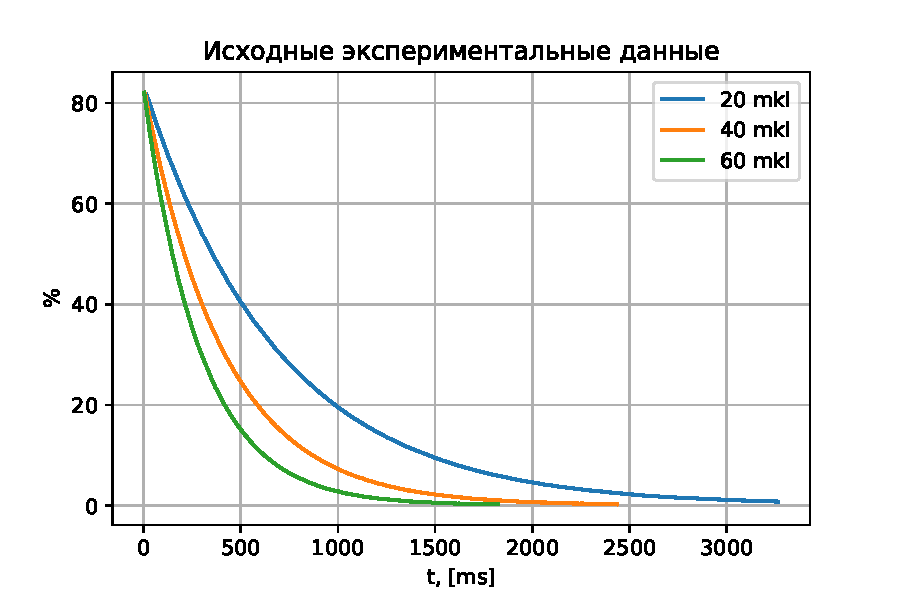
\includegraphics[width=1.2\linewidth]{data/Mn_T_2_exper}
	\caption{}
	\label{fig:mnt2exper}
\end{figure}

Для определения $ T_2 $ построим график $ \ln \left(\dfrac{M}{M_0} \right) = f(\tau) $. Ожидается линейная зависимость с наклоном $ k = -1/T_2 $.

\begin{figure}[!h]
%	\centering
	\hspace{-5em}
	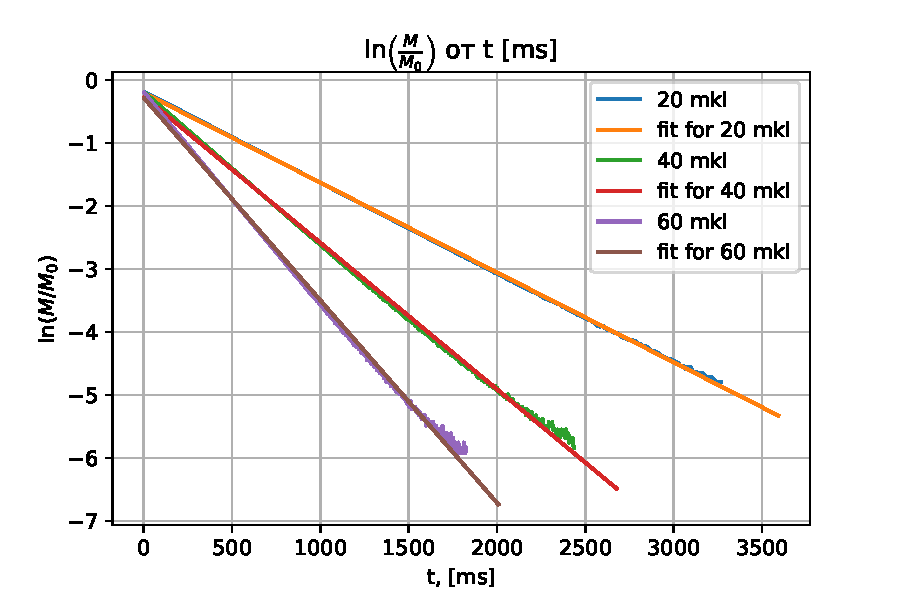
\includegraphics[width=1.2\linewidth]{data/Mn_T_2_reg}
	\caption{}
	\label{fig:mnt2reg}
\end{figure}

Мы находим $ T_2 $ для различных концентраций (см. таблицу \ref{table:all-T})

\subsubsection{Раствор $Na_2 SO_4$}
Производим аналогичные подсчеты и строим те же графики:

\begin{figure}[!h]
	\hspace{-5em}
	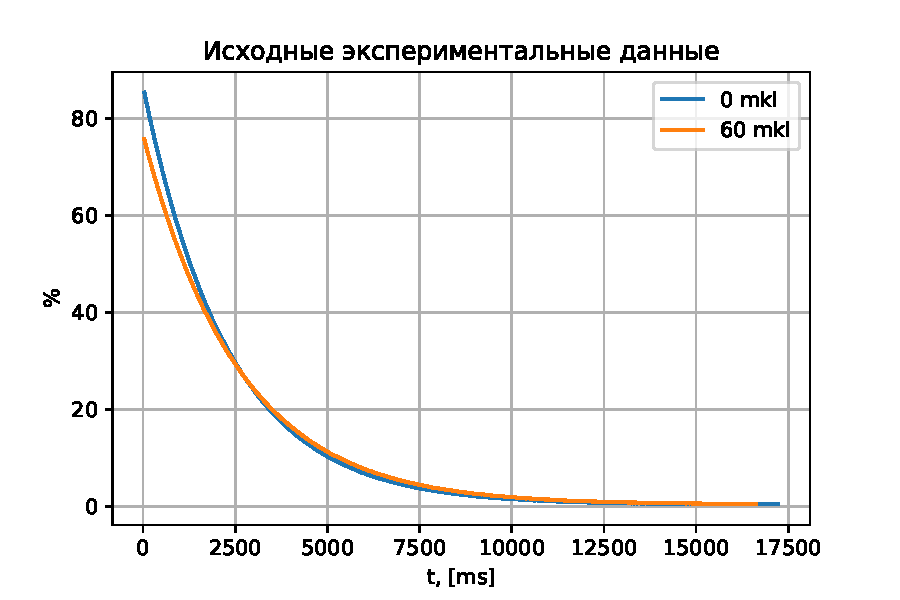
\includegraphics[width=1.2\linewidth]{data/Na_T_2_exper}
	\caption{}
	\label{fig:nat2exper}
\end{figure}

\begin{figure}[!h]
	\hspace{-5em}
	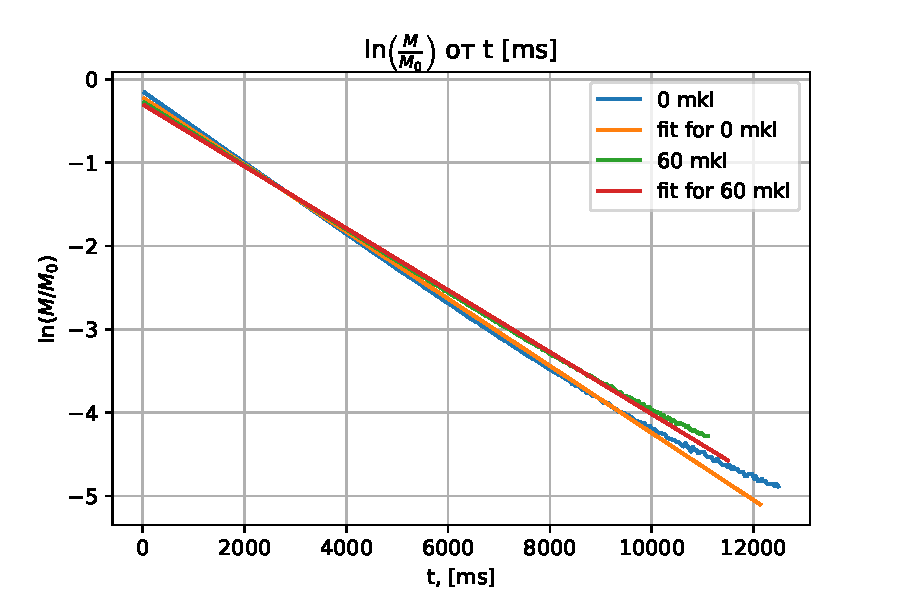
\includegraphics[width=1.2\linewidth]{data/Na_T_2_reg}
	\caption{}
	\label{fig:nat2reg}
\end{figure}



\begin{table}[ht]
	\caption{Сводная таблица с результатами}
	\label{table:all-T}
	\centering
	\begin{tabular}{|l|c|r|r|r|r|}
		\toprule
		Соль &     $V$, мкл &          $T_1$ &          $T_2$ &  $T_2^*$ \\
		\midrule
		$MnSO_4$  	&  20 &  1916.731102 &   700.953789 &  0.68 \\
		$MnSO_4$  	&  40 &  1314.994472 &   429.785639 &  0.68 \\
		$MnSO_4$ 	&  60 &   997.851468 &   310.944742 &  0.68 \\
		$Na_2 SO_4$ &   0 &          --	 &  2563.068945 &  0.68 \\
		$Na_2 SO_4$ &  20 &  2810.293796 &          --  &  0.68 \\
		$Na_2 SO_4$ &  60 &  3305.489338 &  2714.577389 &  0.68 \\
		\bottomrule
	\end{tabular}
\end{table}

\subsection{Обработка результатов}